\chapter{Background}

\section{Paraplegia and Rehabilitation}
Paraplegia is a medical term used to define where a patient loses feeling and/or movement in their lower two limbs. In comparison, quadriplegia (also sometimes known as tetraplegia) is the loss of control in all four limbs. It is important to note that not all feeling/movement needs to be lost in order for someone to be considered paraplegic \cite{IncompleteTraumaticQuadrilegia}. Only 30\% of all paraplegic and quadriplegic patients are considered complete lesions, where there is no sensation and no mobility in the lower limbs \cite{RehabParaplegia}. 

\begin{figure} [h!]
    \centering
    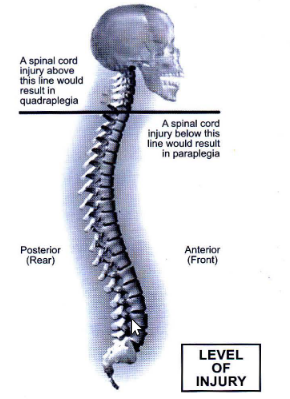
\includegraphics[width=0.5\linewidth]{Figures/Background/ParaQuadInjuryLocs.png}
    \caption{Location of spinal chord injury will determine type of paralysis \cite{RehabParaplegia}}
    \label{fig:ParalysisLocation}
\end{figure}

Paralysis is usually caused by trauma, such as sports injuries, vehicle accidents, or accidental falls, when the spine gets injured (see \autoref{fig:ParalysisLocation}). However, it can also be caused by specific diseases, including multiple sclerosis, amyotrophic lateral sclerosis, stroke, and in specific cases cancer \cite{CausesParaplegia}. Common effects of paraplegia include:
 
\begin{itemize}
    \item Loss of mobility, reflexes, and sensation
    \item Muscular weakness and atrophy
    \item Hormonal variations
    \item Gastrointestinal and bowel/bladder problems
    \item Muscle spasms
    \item Reduced cardiorespiratory fitness and increased likelihood of cardiorespiratory issues
\end{itemize}

\todo[]{Talk about skin problems in paralysis patients} 

Rehabilitation can play a key role in reducing these side effects in patients who experience paraplegia. Mainly, physical therapy for paralysis patients focus on three main types of exercises: stretching, strengthening, and aerobic. Additionally, paralysis patients may go through gait training with the assistance of medical devices.

\subsection{Physical Therapy for Paralysis Patients}

\begin{figure}[ht!]
    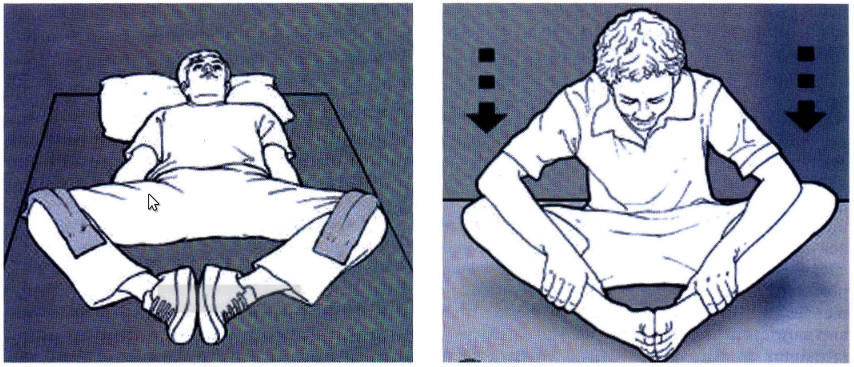
\includegraphics[width=\linewidth]{Figures/Background/BilateralAdductorStretch.png}
    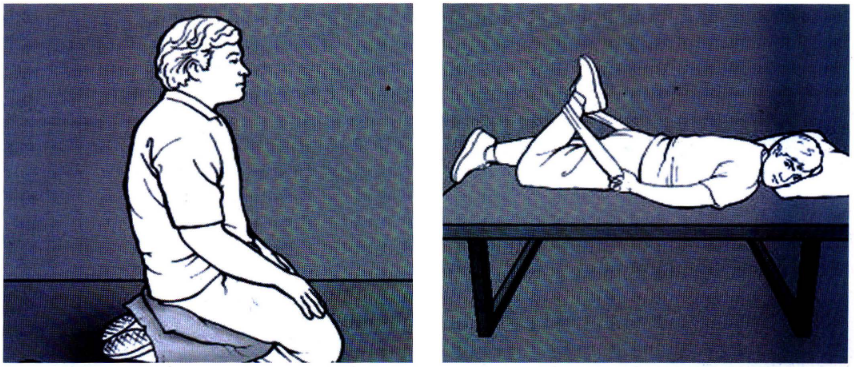
\includegraphics[width=\linewidth]{Figures/Background/QuadricepsStretch.png}
    \caption{Bilateral Adductor Stretches (top) and Quadriceps Stretches (bottom) for paraplegic and quadriplegic patients \cite{RehabParaplegia}}
    \label{fig:ParaplegiaStretches}
\end{figure}

\subsubsection{Stretching}
Stretching is considered one of the most important exercises \cite{RehabParaplegia}, more-so than any other form of exercise because it can be done often and at home. Carefully designed exercises (like seen in \autoref{fig:ParaplegiaStretches}) can improve flexibility, reduce muscle spasms, reduce the chance of injury, and relieve contractures \cite{ParalysisStretchingWeightLoadingPMID} \cite{ParalysisStretchingHarvey} \cite{ParalysisStretchingMichigan}. Some common stretches include bilateral adductor stretches, quadriceps stretches, and hip flexor stretches.

\subsubsection{Cardiorespiratory and Cardiovascular Training}
Due to the difficulty of exercise, cardiovascular and cardiorespiratory activities are also very important to maintain health in paralysis patients. Aerobic exercises can increase energy levels, improve lung and heart function, control body weight, and reduce fatigue \cite{RehabParaplegia} \cite{AerobicCapacityParaplegia}. A study showed that patients who suffer from neuromuscular deficiencies such as paraplegia suffered decreasing VO\textsubscript{2} max compared to control subjects with no issues \cite{AerobicCapacityParaplegia}. VO\textsubscript{2} max a common metric that measures the maximum rate of oxygen utilization during heavy exercise. Combination of the upper body and lower body in paraplegic patients can strengthen the paralyzed limbs while also activating healthy limbs. Some researchers have even proposed introducing wheelchair racing as a sport in an effort to help with rehabilitation after paraplegia \cite{WheelchairRacingParaplegia}.

\subsubsection{Strength Training}
Improving strength in muscles may actually partially reverse the loss of mobility in partially paralyzed patients, while also improving muscle tone \cite{AerobicCapacityParaplegia} and preventing bone atrophy \cite{ParalysisStretchingWeightLoadingPMID}. This type of exercise can be split into two major regions: training of affected limbs and muscles, and the training of non-affected regions. Affected limbs can benefit from an increase in mobility and definition, and can generally reduce the likelihood of muscular atrophy. Additionally, strong hip and leg muscles in partially paraplegic patients can help in gait training and increase the possibility of usage in life. On the other side, increasing or maintaining strength in unaffected regions can help with quality of life improvement. Often, paraplegic patients may elect to use crutches or canes as an assisted mobility device in the real world. Increasing arm/shoulder strength and endurance will also increase capability for patients to use some of these assisted devices. Finally, back and abdomen muscles are very important to strengthen to maintain posture and improve gait performance \cite{TrunkMuscleLoadingParaplegia}. 

\subsubsection{Hydrotherapy}
Hydrotherapy (exercising in water) is a notable way for patients suffering from paraplegia to better strengthen muscles and improve cardiovascular health. Due to similar buoyancy, water can reduce the effects of gravity without any external assistive devices. At the same time, the increased density of the water (in comparison to air) creates a natural resistance without the use of weights or elastics. Therefore, hydrotherapy is used in paraplegic patients to increase muscle power, increase endurance, and even help with gait training (see \autoref{sec:GaitTraining}). In minor cases of paralysis, some patients even use swimming as a way to exercise \cite{RehabParaplegia} \cite{BenefitsOfHydrotherapy}.

\subsection{Gait Training}
\label{sec:GaitTraining}

Gait training has become the best way to improve motor functions in those who have partially or fully lost mobility in their legs and torso. The premise of this exercise is to have patients do similar movements to what one would do without their disability, like walking and climbing stairs. Essentially, the goal is to help the patient relearn the gaits they previously knew. Spinal neuronal circuits degrade quickly - in just a year, they can lose most of their potency, essentially unlearning any gait abilities the patient had in the past \cite{GaitTrainingClinical} \cite{RehabParaplegia} \cite{TrunkMuscleLoadingParaplegia}. Gait training can help reconnect the broken spinal neurons, and improve motor function and balance in a patient. In fact, several studies have show that some patients with full spinal chord injuries have been able to recover part or even all of their walking capabilities through gait training \cite{GaitTrainingClinical} \cite{ImprovingGaitAdaptabilityInPatients}! 
\footnote{There is significant research in the benefits of gait training for paraplegic and quadriplegic patients. Not all prior work is cited here.} 

\subsubsection{Use of Assistive Devices for Gait Training}
Since most patients suffering from paralysis won't be able to hold themselves up, there have been many different proposals to compensate for gravity. At lower levels of paralysis, canes, walkers, and other walking assisted devices can help. Hydrotherapy has also been used with gait training due to the similar densities of humans and water \cite{BenefitsOfHydrotherapy}. With more serious cases of paralysis, robotic solutions and other active orthotics have been proposed and used in clinical settings.

Standard solutions like canes and walkers will only work for patients with mild paralysis. Canes are designed to support only 25\% of body weight \cite{RehabParaplegia}. They can also be fairly unstable, since they usually only have at most 4 points of contact with a very small ground contact area. Walkers are better than canes, since they can support up to 50\% of body weight \cite{RehabParaplegia}. However, canes, walkers, and crutches have one downside: the required upper-body strength. Mild lower-limb paralysis cases usually can benefit from these inexpensive tools to help with gait training. However most patients will struggle holding themselves up during gait training.

\begin{figure} [h!]
    \centering
    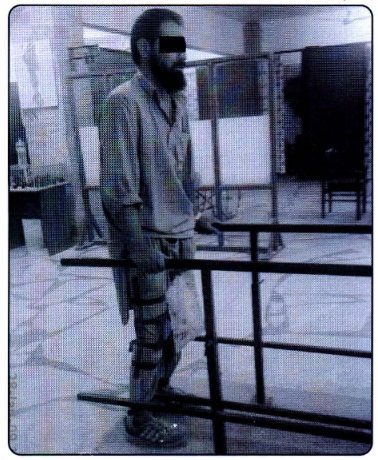
\includegraphics[width=0.5\linewidth]{Figures/Background/SplintsDemo.png}
    \caption{Patient using basic splint orthosis \cite{RehabParaplegia}}
    \label{fig:SplintsDemo}
\end{figure}

Orthosis are the next level up in assistive devices. They can come in many different shapes and can be designed to fit a patient's progress. At the lowest levels are specialty splints or braces (seen in \autoref{fig:SplintsDemo}) that can help keep joints locked or reduce load of a joint through passive springs. These solutions often cost very little in material, and apply normal loads on the user's skeletal system - helping to prevent bone atrophy. Actively powered orthosis also exist with various levels of research and clinical trials (see \autoref{sec:OtherExos}), and can be separated in two major groups. 

\begin{figure}[h!]
    \centering
    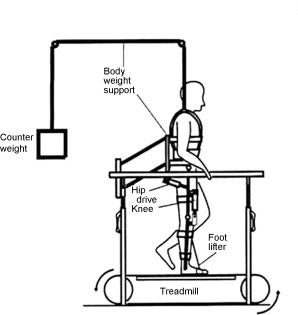
\includegraphics[width=0.5\textwidth]{Figures/Background/ExoSeparateGravityComp.png}
    \caption{Comparison between an exoskeleton with active gravity compensation (left) and an exoskeleton with passive gravity compensation (right) \cite{GaitTrainingClinical}}
    \label{fig:ExoTypesGCSCompared}
\end{figure}
\todo[]{Add additional figure of an active GCS exo}

Actively compensating exoskeletons (see left image in \autoref{fig:ExoTypesGCSCompared}) are orthosis devices that use various types of actuators, sensors, and gait controllers to help keep patients standing and walking with little to no strength required (from the patient). These types of exoskeletons use up a significant amount of energy, since they must essentially do all the physical work that leg muscles would normally do. This usually means very powerful actuators and motors with precise and stable control, and large batteries (which add to overall weight) or a large/long tether. Such power increases the overall flexibility of the system, however, at a cost. It also increases complexity of the control software, and introduces a safety risk of attaching powerful actuators to patient limbs.

To mitigate some of these risks, some solutions separate the exoskeleton and the gravity compensation (see right image in \autoref{fig:ExoTypesGCSCompared}). A separate mechanical system supports the weight of the user usually through a counterweight system or a gantry of some sort. This allows for the actuator in the exoskeleton orthosis to be weaker or power (current) limited to prevent injury in case of a malfunction. However, such systems are much more limited in their uses, since the power is hardware limited and more infrastructure is needed to use the device. Additionally, any actively compensating exoskeleton orthosis can be current limited and be used with a mechanical gravity compensation system. 

However, one of the biggest struggles with orthoses is the dermatological problems that they may cause. As explained earlier, patients suffering from paralysis are at an increased risk of developing skin complications \cite{DermatologicalIssuesParalysis}. This can be at least partially attributed to reduced sensitivity in paralyzed areas of the body. Therefore, any assisted devices that attach to a patient's skin should accurately follow the natural trajectory of the skin to avoid unnecessary rubbing.

\subsubsection{Robotics for Paralysis Rehabilitation}
Robotics have a very large opportunity to improve the rehabilitation process in paraplegic patients. Clinical research in using robotic orthosis for gait training and other rehabilitation exercises show positive improvement in most patients when considering quality of life \cite{GaitTrainingBenefitsRoboticsWalkbot} \cite{RoboticGaitTraining}. 
\improvement{Add more to this part}

\section{Research in the Human Knee and Applicable Orthoses}

\subsection{Knee Orthoses Design Requirements}

\section{Previous work on Exoskeleton Orthosis}
\label{sec:OtherExos}
Exoskeletons are an interesting application to help those with walking disabilities rehabilitate and exercise their muscles.

\subsection{H2}

\subsection{ReWalk}

\subsection{EKSO}

\subsection{Indigo}

\subsection{KINESIS}

\subsection{HAL}

\section{WPI LARRE Exoskeleton}
% LARRE Stands for Legged Articulated Robotic Rehabilitation Exoskeleton 